%!TEX root = ../thesis.tex
%*******************************************************************************
%*********************************** Research Timelines *****************************
%*******************************************************************************



\chapter{Research Timeline}  %Title of the Research Timeline

\ifpdf
    \graphicspath{{ResearchTimeline/Figs/Raster/}{ResearchTimeline/Figs/PDF/}{ResearchTimeline/Figs/}}
\else
    \graphicspath{{ResearchTimeline/Figs/}{ResearchTimeline/Figs/}}
\fi

% Please add the following required packages to your document preamble:
% \usepackage{graphicx}
\begin{table}[]
    \resizebox{\columnwidth}{!}{%
    \begin{tabular}{|l|l|}
    \hline
    \textbf{CPP} & \textbf{Conference}                                                                                        \\ \hline
    March        & ISMM (International Symposium on Memory Management)                                                        \\ \hline
    April        & SOSP (Symposium on Operating Systems Principles)                                                           \\ \hline
    June         & ASPLOS (International Conference on Architectural Support for Programming Languages and Operating Systems) \\ \hline
    September    & EuroS\&P (European Symposium on Security and Privacy)                                                      \\ \hline
    October      & EuroSys                                                                                                    \\ \hline
    December     & OSDI (USENIX Symposium on Operating Systems Design and Implementation)                                     \\ \hline
    \end{tabular}%
    }
    \caption{List of relavent conferences to submit for the following PhD expirements.}
    \end{table}

This PhD plan outlines a comprehensive research project to explore, implement, and evaluate FAT-Pointer based range addressing mechanisms across various systems, 
including ARM with hugepages, RISC-V, and Uni-Kernels.The research is structured into several phases, each focusing on distinct aspects of the FAT-Pointer based range address
mechanism. Each expirement constitutes a chapter in the final thesis.

\begin{figure}[h]
    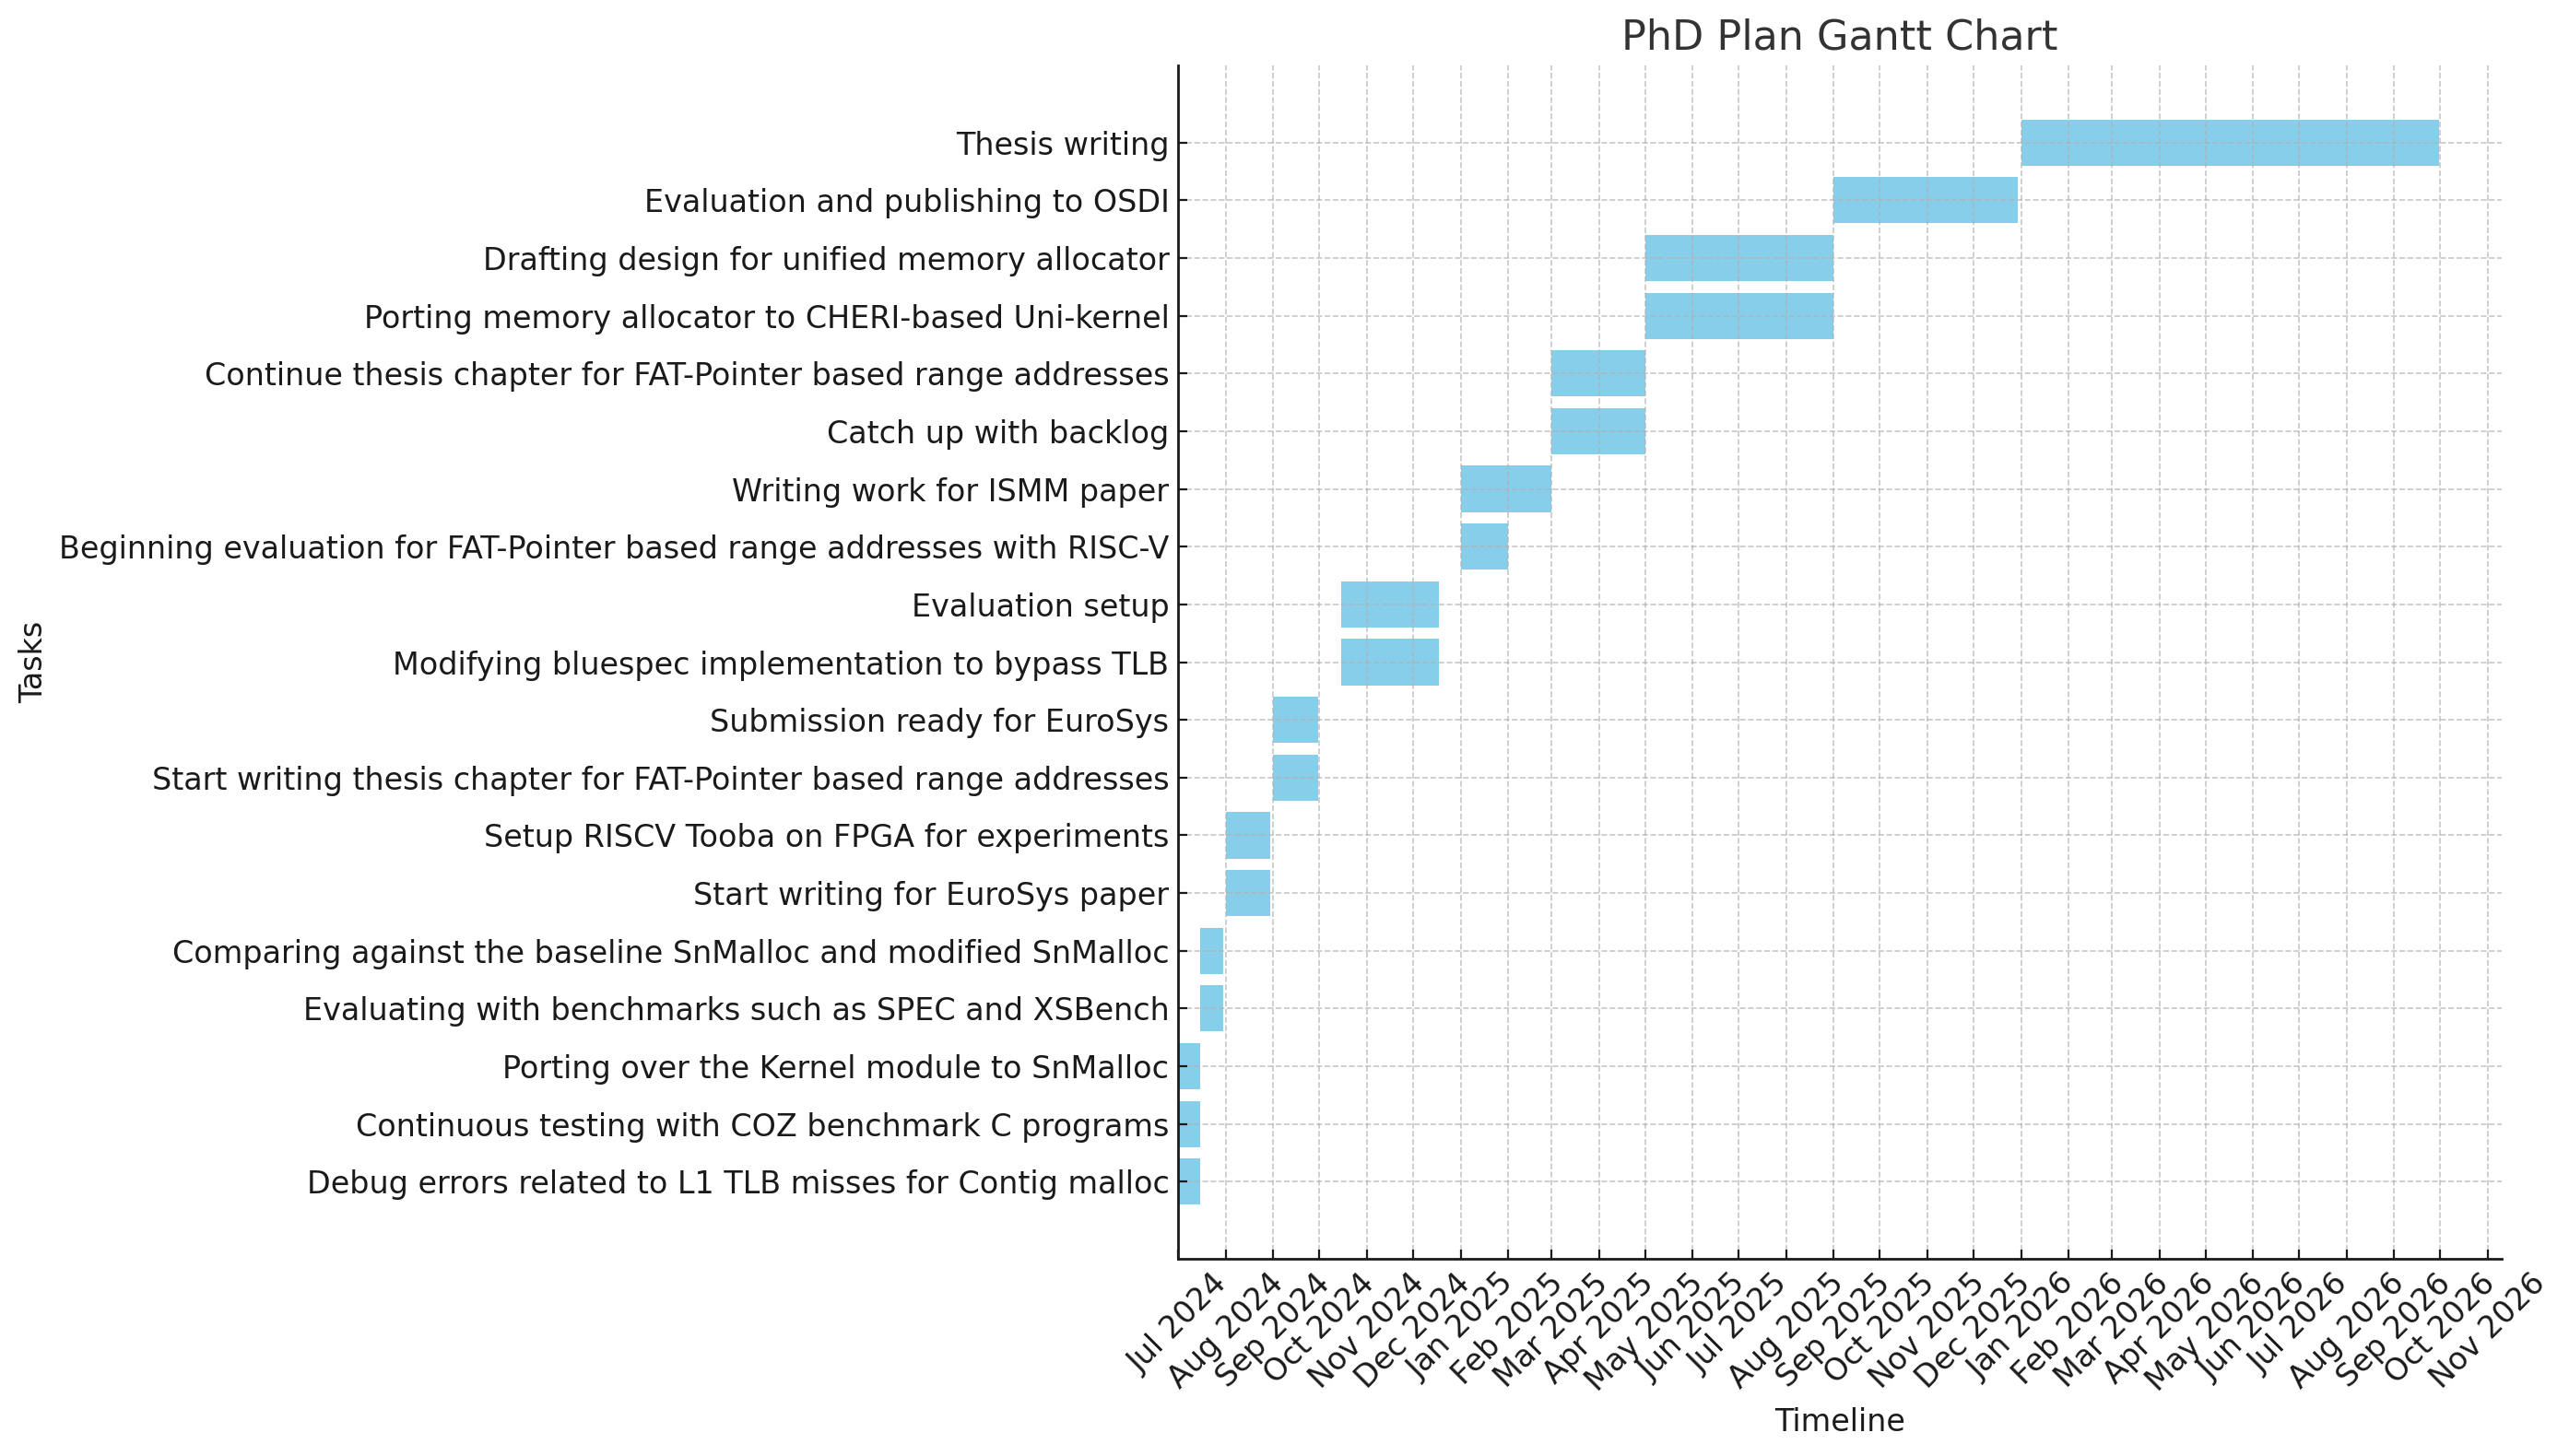
\includegraphics[width=0.8\textwidth]{GnattChart.png}
    \caption{PhD plan Gnatt Chart}
    \label{fig:RMM}
  \end{figure}

\section{FAT-Pointer based range addresses}
\subsection{July 1th - July 15th (2024)}
    \subsubsection{Debug Errors Related to L1 TLB Misses for Contiguous malloc}
    \begin{enumerate}
        \item Investigate the cause of L1 TLB misses when using contiguous memory allocation with the FAT-Pointer mechanism.
        \item Utilize debugging tools and techniques to identify specific issues within the memory management unit (MMU) and translation lookaside buffer (TLB).
        \item Implement and test fixes to ensure efficient TLB usage and reduced misses.
    \end{enumerate}
    \subsubsection{Continous testing with COZ benchmark C programs}
    \begin{enumerate}
        \item Run COZ benchmark C programs to evaluate the performance and correctness of the FAT-Pointer based range addressing.
        \item Analyze the benchmarking results to identify potential performance bottlenecks.
        \item Refine the FAT-Pointer implementation based on feedback from the benchmark tests.
    \end{enumerate}
    \subsubsection{Port the Kernel Module to SnMalloc, the Default CHERIBSD Kernel Allocator}
    \begin{enumerate}
        \item Modify the existing ported contig kernel module to be compatible with SnMalloc.
        \item Test the ported module to verify its functionality and performance.
    \end{enumerate}

\subsection{July 15th - July 30th (2024)}
\subsubsection{Evaluate Performance Using Benchmarks Such as SPEC and XSBench}
\begin{enumerate}
    \item Set up and run SPEC and XSBench benchmarks to assess the performance of the FAT-Pointer based range addressing.
    \item Collect and analyze performance metrics to gauge the impact of the FAT-Pointer mechanism.
\end{enumerate}
\subsubsection{Compare Results Against the Baseline SnMalloc and Modified SnMalloc Memory Allocator}
\begin{enumerate}
    \item Perform comparative analysis between the default SnMalloc, modified SnMalloc, and FAT-Pointer based allocator.
    \item Document performance improvements or regressions to understand the benefits and drawbacks of the FAT-Pointer based range addresses implementation.
\end{enumerate}

\subsection{August 1st - August 30th (2024)}
\subsubsection{Begin Writing the Paper for EuroSys}
\begin{enumerate}
    \item Start drafting the EuroSys paper focusing on the design, implementation, and performance evaluation of the FAT-Pointer based range addressing.
    \item Ensure the setup is capable of running relevant tests and benchmarks for evaluating the FAT-Pointer mechanism on RISCV architecture.
\end{enumerate}

\subsection{September 1st - September 30th (2024)}
\subsubsection{Start Writing the Thesis Chapter on FAT-Pointer Based Range Addresses}
\begin{enumerate}
    \item Begin compiling and organizing research findings and insights into a comprehensive thesis chapter.
    \item Provide detailed explanations of the design, implementation, and performance evaluations conducted.
\end{enumerate}
\subsubsection{Prepare the Submission for EuroSys}
\begin{enumerate}
    \item Finalize the EuroSys paper based on feedback and revisions.
    \item Ensure all necessary documentation and supplementary materials are ready for submission.
\end{enumerate}

\section{FAT-Pointer based range addresses with RISC-V}
\subsection{October 15th - December 18th (2024)}
\subsubsection{Modify the Bluespec Implementation to Bypass the TLB}
\begin{enumerate}
    \item Engineer modifications in the Bluespec implementation to enable bypassing the TLB.
    \item Test the changes to ensure they achieve the desired effect and maintain system stability.
\end{enumerate}
\subsubsection{Set Up the Evaluation Environment}
\begin{enumerate}
    \item Prepare the necessary hardware and software environment for evaluating the modified Bluespec implementation.
    \item Ensure all tools and benchmarks are properly configured for accurate performance measurements.
\end{enumerate}

\subsection{January 1st - Feburary 1st (2025)}
\subsubsection{Begin the Evaluation of FAT-Pointer Based Range Addresses with RISC-V}
\begin{enumerate}
    \item Conduct a thorough evaluation of the FAT-Pointer mechanism on the RISC-V architecture.
    \item Collect performance data and analyze the results to assess the impact of the FAT-Pointer range address based RISCV implementation.
\end{enumerate}
\subsubsection{Start Writing the Paper for ISMM}
\begin{enumerate}
    \item Begin drafting the ISMM paper, focusing on the technical details and evaluation results of the FAT-Pointer implementation on RISC-V.
    \item Highlight the innovations and contributions of this work to the field.
\end{enumerate}

\subsection{Feburary 1st - March 1st (2025)}
\subsubsection{Start Writing the Paper for ISMM}
\begin{enumerate}
    \item Refine the ISMM paper based on initial drafts and feedback.
    \item Ensure the paper thoroughly covers the research, findings, and implications.
\end{enumerate}

\subsection{March 1st - May 1st (2025)}
\subsubsection{Catch Up on Any Backlog Tasks}
\begin{enumerate}
    \item Address any remaining tasks or issues that were postponed earlier.
    \item Ensure all aspects of the research project are up to date.
\end{enumerate}
\subsubsection{Continue Writing the PhD Thesis Chapter on FAT-Pointer Based Range Addresses}
\begin{enumerate}
    \item Expand on the thesis chapter with detailed explanations of recent findings and evaluations.
    \item Ensure the chapter provides a comprehensive overview of the FAT-Pointer research.
\end{enumerate}

\section{FAT-Pointer based range addresses with Uni-kernels}
\subsection{May 1st - September 1st (2025)}
\subsubsection{Catch Up on Any Backlog Tasks}
\begin{enumerate}
    \item Adapt the FAT-Pointer based memory allocator for use with a CHERI-based Uni-Kernel.
    \item Test the ported allocator to ensure compatibility and performance within the Uni-Kernel environment.
\end{enumerate}
\subsubsection{Draft a Design for a Unified Memory Allocator}
\begin{enumerate}
    \item Develop a design for a unified memory allocator that can be used by both the kernel and applications in the Uni-Kernel.
    \item Document the design considerations, challenges, and proposed solutions.
\end{enumerate}
\subsection{September 1st - December 30th (2025)}
\subsubsection{Perform Evaluation and Prepare a Publication for OSDI}
\begin{enumerate}
    \item Conduct performance and functionality evaluations of the unified memory allocator.
    \item Compile results and draft a paper for submission to OSDI, highlighting the key contributions and findings.
\end{enumerate}
\subsection{Janurary 1st - September 30th (2026)}
\subsubsection{Focus on Writing the PhD Thesis}
\begin{enumerate}
    \item Dedicate time to writing and refining the PhD thesis.
    \item Ensure all research chapters are complete, well-organized, and thoroughly reviewed.
\end{enumerate}


% PhD Plan for FAT-Pointer Based Range Addresses
% July 1st - July 15th, 2024
% Debug Errors Related to L1 TLB Misses for Contiguous malloc

% Investigate the cause of L1 TLB misses when using contiguous memory allocation with the FAT-Pointer mechanism.
% Utilize debugging tools and techniques to identify specific issues within the memory management unit (MMU) and translation lookaside buffer (TLB).
% Implement and test fixes to ensure efficient TLB usage and reduced misses.
% Conduct Continuous Testing with COZ Benchmark C Programs

% Run COZ benchmark C programs to evaluate the performance and correctness of the FAT-Pointer based range addressing.
% Analyze the benchmarking results to identify potential performance bottlenecks.
% Refine the FAT-Pointer implementation based on feedback from the benchmark tests.
% Port the Kernel Module to SnMalloc, the Default CHERIBSD Kernel Allocator

% Modify the existing kernel module to be compatible with SnMalloc.
% Ensure seamless integration with the CHERIBSD operating system.
% Test the ported module to verify its functionality and performance.
% July 15th - July 30th, 2024
% Evaluate Performance Using Benchmarks Such as SPEC and XSBench

% Set up and run SPEC and XSBench benchmarks to assess the performance of the FAT-Pointer based range addressing.
% Collect and analyze performance metrics to gauge the impact of the FAT-Pointer mechanism.
% Compare Results Against the Baseline SnMalloc and Modified SnMalloc Memory Allocator

% Perform comparative analysis between the default SnMalloc, modified SnMalloc, and FAT-Pointer based allocator.
% Document performance improvements or regressions to understand the benefits and drawbacks of the FAT-Pointer implementation.
% August 1st - August 30th, 2024
% Begin Writing the Paper for EuroSys

% Start drafting the EuroSys paper focusing on the design, implementation, and performance evaluation of the FAT-Pointer based range addressing.
% Highlight key findings, methodology, and the significance of the research.
% Set Up RISCV Tooba on FPGA for Upcoming Experiments

% Install and configure the RISCV Tooba platform on an FPGA to facilitate future experiments.
% Ensure the setup is capable of running relevant tests and benchmarks for evaluating the FAT-Pointer mechanism on RISCV architecture.
% September 1st - September 30th, 2024
% Start Writing the Thesis Chapter on FAT-Pointer Based Range Addresses

% Begin compiling and organizing research findings and insights into a comprehensive thesis chapter.
% Provide detailed explanations of the design, implementation, and performance evaluations conducted.
% Prepare the Submission for EuroSys

% Finalize the EuroSys paper based on feedback and revisions.
% Ensure all necessary documentation and supplementary materials are ready for submission.
% FAT-Pointer Based Range Addresses with RISC-V
% October 15th - December 18th, 2024
% Modify the Bluespec Implementation to Bypass the TLB

% Engineer modifications in the Bluespec implementation to enable bypassing the TLB.
% Test the changes to ensure they achieve the desired effect and maintain system stability.
% Set Up the Evaluation Environment

% Prepare the necessary hardware and software environment for evaluating the modified Bluespec implementation.
% Ensure all tools and benchmarks are properly configured for accurate performance measurements.
% January 1st - February 1st, 2025
% Begin the Evaluation of FAT-Pointer Based Range Addresses with RISC-V

% Conduct a thorough evaluation of the FAT-Pointer mechanism on the RISC-V architecture.
% Collect performance data and analyze the results to assess the impact of the FAT-Pointer implementation.
% Start Writing the Paper for ISMM

% Begin drafting the ISMM paper, focusing on the technical details and evaluation results of the FAT-Pointer implementation on RISC-V.
% Highlight the innovations and contributions of this work to the field.
% February 1st - March 1st, 2025
% Continue Writing the ISMM Paper
% Refine the ISMM paper based on initial drafts and feedback.
% Ensure the paper thoroughly covers the research, findings, and implications.
% March 1st - May 1st, 2025
% Catch Up on Any Backlog Tasks

% Address any remaining tasks or issues that were postponed earlier.
% Ensure all aspects of the research project are up to date.
% Continue Writing the PhD Thesis Chapter on FAT-Pointer Based Range Addresses

% Expand on the thesis chapter with detailed explanations of recent findings and evaluations.
% Ensure the chapter provides a comprehensive overview of the FAT-Pointer research.
% FAT-Pointer Based Range Addresses with Uni-Kernels
% May 1st - September 1st, 2025
% Port the Memory Allocator to a CHERI-Based Uni-Kernel

% Adapt the FAT-Pointer based memory allocator for use with a CHERI-based Uni-Kernel.
% Test the ported allocator to ensure compatibility and performance within the Uni-Kernel environment.
% Draft a Design for a Unified Memory Allocator

% Develop a design for a unified memory allocator that can be used by both the kernel and applications in the Uni-Kernel.
% Document the design considerations, challenges, and proposed solutions.
% September 1st - December 30th, 2025
% Perform Evaluation and Prepare a Publication for OSDI
% Conduct performance and functionality evaluations of the unified memory allocator.
% Compile results and draft a paper for submission to OSDI, highlighting the key contributions and findings.
% January 1st - September 30th, 2026
% Focus on Writing the PhD Thesis
% Dedicate time to writing and refining the PhD thesis.
% Ensure all research chapters are complete, well-organized, and thoroughly reviewed.
    
% \section{FAT-Pointer based range addresses}

% \subsection{Month 1: July 2024}
% \subsubsection{Week 2 (July 8 - July 14)}
% Benchmarking:
% Porting over the current Malloc to Benchmarks such as (Benchmark examples).
% Select a suitable memory-intensive application (e.g., database, scientific computation software).
% Establish baseline performance metrics with standard page sizes.
% Document the baseline TLB miss rates, memory access latency, and application performance.

% Week 3 (July 15 - July 21)
% Data Collection:
% Plot graphs based on the new Benchmarks executed.

% Week 4 (July 22 - July 28)

% Data Analysis:
% Analyze the initial data to identify trends and patterns.
% Compare the results with baseline metrics.
% Prepare an interim report on initial findings.
% Month 2: August 2024
% Week 1 (July 29 - August 4)

% Optimization and Troubleshooting:
% Optimize the application and system configuration for better utilization of huge pages.
% Address any issues identified in the initial testing phase.
% Conduct additional testing to refine the performance metrics.
% Week 2 (August 5 - August 11)

% Advanced Testing:
% Test different configurations (e.g., different huge page sizes, mixed page sizes).
% Collect comprehensive performance data for each configuration.
% Ensure repeatability and consistency in the results.
% Week 3 (August 12 - August 18)

% Comparative Analysis:
% Perform a comparative analysis of the performance with different huge page configurations.
% Evaluate the impact of huge pages on TLB miss rates and memory access latency.
% Document the findings in a detailed report.
% Week 4 (August 19 - August 25)

% Further Optimization and Validation:
% Validate the results by repeating key experiments.
% Fine-tune the application and system settings based on previous findings.
% Ensure that the results are statistically significant.
% Month 3: September 2024
% Week 1 (August 26 - September 1)

% Documentation:
% Start drafting the final report and thesis chapter on the experiment.
% Include detailed methodology, data analysis, results, and discussion.
% Week 2 (September 2 - September 8)

% Review and Refinement:
% Review the draft report and thesis chapter.
% Incorporate feedback from advisors and peers.
% Refine the analysis and discussion sections.
% Week 3 (September 9 - September 15)

% Final Report and Presentation Preparation:
% Finalize the report and thesis chapter.
% Prepare a presentation on the findings.
% Schedule a review meeting with the advisory committee.
% Week 4 (September 16 - September 22)

% Final Review and Submission:
% Present the findings to the advisory committee.
% Make final adjustments based on feedback.
% Submit the final report and thesis chapter.
% Plan the next steps for follow-up experiments or further research.
% Week 5 (September 23 - September 30)

% EuroSys Submission Preparation:
% Format the findings into a conference paper suitable for EuroSys.
% Ensure all submission guidelines are followed.
% Prepare supplementary materials (e.g., data sets, code repositories) if required by the conference.

% \begin{figure}[htbp!] 
%   \centering    
%   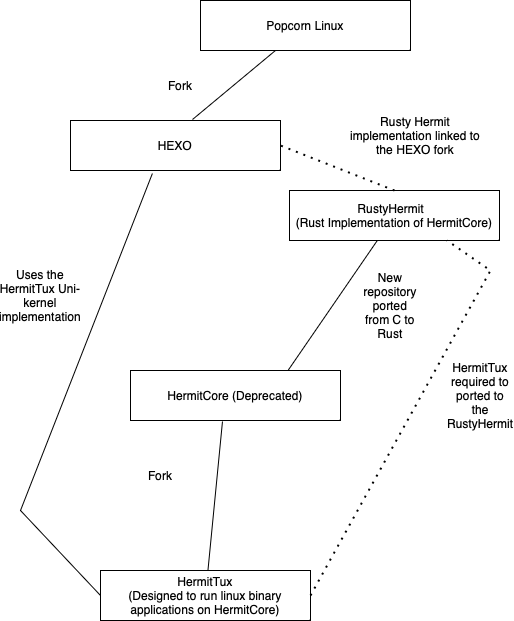
\includegraphics[width=0.6\textwidth]{PlannerActivity}
%   \caption[High-level overview of the porting efforts]{High-level overview of the porting efforts}
%   \label{fig:PlannerPorting}
%   \end{figure}

% Before starting a heavy discussion of the plan and experiment a few things that should cleared out before starting would be 
% the higher overview of the experiment and why certain porting efforts are required. The Segments would be classified into: 
% \begin{enumerate}
%   \item Porting the Unikernel implementation 
%   \item Porting CheriBSD to a Uni-kernel
% \end{enumerate}

% \subsubsection{Porting the Unikernel implementation}
% The Uni-kernel implementation used for the following PhD would be RustyHermit 
% which is Rust implementation of the Uni-kernel project Hermit-core. The reason 
% RustyHermit was selected is because the Hermit-core project is deprecated and 
% the recent version of the project is the RustyHermit repo. To give a better 
% background the HEXO paper \cite{HEXO} which uses Popcorn Linux to offload 
% tasks to a potato machine (i.e raspberry pi) which uses the HermitTux Uni-kernel (This 
% is a fork for the Hermit-core Uni-kernel). The HermitTux fork of HermitCore is used to 
% run Linux ABI binary files on a Uni-kernel. To ensure we can continue working with the
% planned experiments. It would recommended to port HermitTux to RustyHermit to ensure we 
% can sync the new version of HermitTux with the latest changes from RustyHermit. Fig ~\ref{fig:PlannerPorting}
%  provides the visual description of the following paragraph. 

% \subsubsection{Porting CheriBSD to a Uni-kernel}
% The selected TAG based architecture would be CHERI due to ease to acquiring of hardware 
% for performance (i.e the ARM based CHERI morello). The official supported OS for 
% the CHERI hardware is the CheriBSD \cite{CHERIBSD}. While doing experiments it 
% would save a lot of time initially just porting the required kernel modules to 
% RustyHermit.

% \subsubsection{Hardware requirements}
% Initially from the month of January 2023 they would tested locally on 
% my personal of machine, but over the semester 
% \begin{enumerate}
%   \item 1 Cheri Morello machine 
%   \item 2 Bare-metal x86 machines
%   \item 2 FPGAs (For testing new architectures)
%   \item 2 ARM based machines
%   \item Rack space for setting up the machines 
% \end{enumerate}

% \subsubsection{The tasks are split into the following tags:}
% \begin{enumerate}
%   \item Porting 
%   \item Setup
%   \item Development
%   \item Exploration 
%   \item Technical discussion 
%   \item Writing
%   \item Testing
%   \item Publishing
%   \item Thesis
%   \item Break
%   \item Other
% \end{enumerate}

% % \subsection{More context}
% % This section is split by a month by month planner to help keep tracks of tasks. 

% \subsection{Year 2}
% This section is split by a month by month planner to help keep tracks of tasks. 
% % \begin{landscape}
% \begin{figure}[htbp!] 
%   \centering    
%   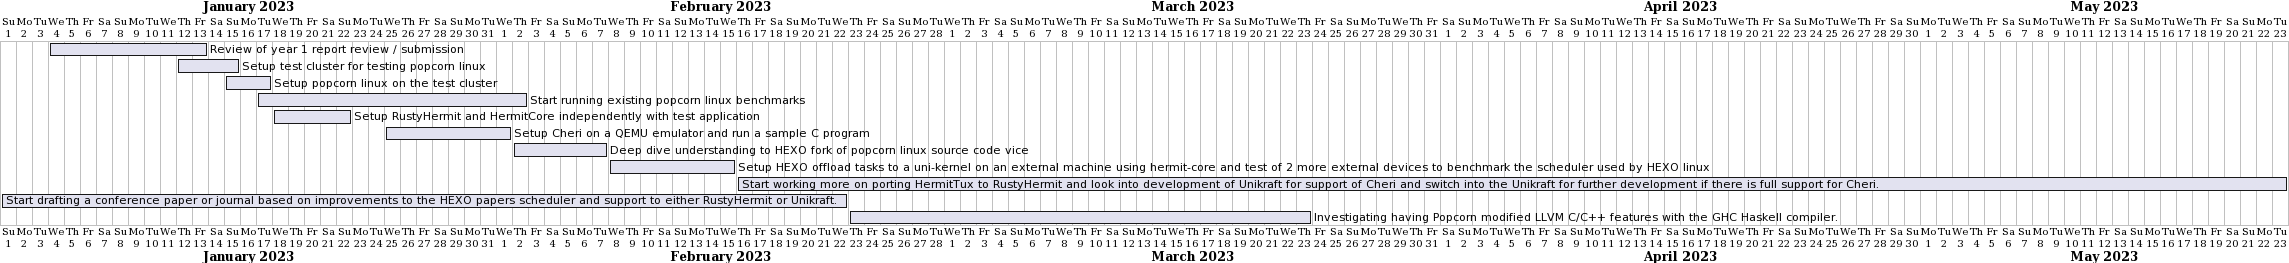
\includegraphics[width=1.2\textwidth]{gnatt-1}
%   \caption[Gantt Chart till summer 2023]{Gantt Chart till summer 2023}
%   \label{fig:Gantt Chart}
%   \end{figure}
% % \end{landscape}
% % \begin{landscape}
%   \begin{figure}[htbp!] 
%     \centering    
%     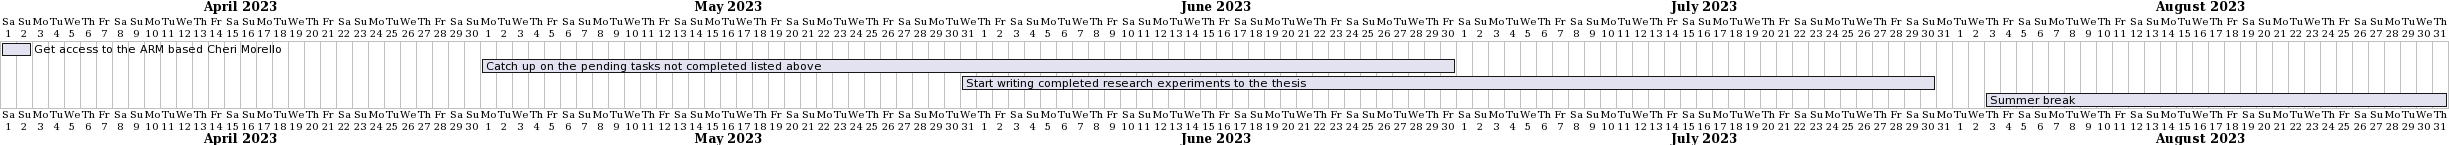
\includegraphics[width=1.2\textwidth]{gnatt-2}
%     \caption[Gantt Chart till summer 2023]{Gantt Chart till summer 2023}
%     \label{fig:Gantt Chart}
%     \end{figure}
%   % \end{landscape}
%   % \begin{landscape}
%     \begin{figure}[htbp!] 
%       \centering    
%       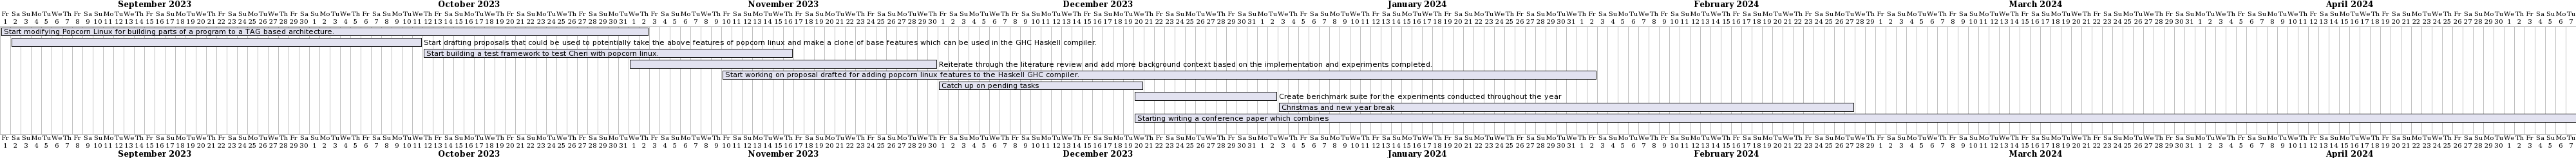
\includegraphics[width=1.2\textwidth]{gnatt-3}
%       \caption[Gantt Chart till summer 2023]{Gantt Chart till summer 2023}
%       \label{fig:Gantt Chart}
%       \end{figure}
%     % \end{landscape}  

% \subsubsection{January 2023}
% The high level overview being that most of the setups for the upcoming experiments
% are complete. 
% \begin{enumerate}
%     \item (\(Review\)) Review of year 1 report submitted 
%     \item (\(Setup\)) Setup test cluster for testing popcorn linux 
%     \item (\(Setup\)) Setup popcorn linux on the test cluster
%     \item (\(Testing\)) Start running existing popcorn linux benchmarks 
%     \item (\(Setup\)) Setup RustyHermit and HermitCore independently with test application 
%     \item (\(Setup\)) Setup Cheri on a QEMU emulator and run a sample C program 
%   \end{enumerate} 


%   \subsubsection{February 2023}
%   \begin{enumerate}
%     \item (\(Exploration\)) Deep dive understanding to HEXO fork of popcorn linux source code vice.
%     \item (\(Setup\)) Setup HEXO offload tasks to a uni-kernel on an external machine using hermit-core 
%     and test of 2 more external devices to benchmark the scheduler used by HEXO linux. 
%     \item (\(Porting\)) Start working more on porting HermitTux to RustyHermit and look into 
%     development of Unikraft for support of Cheri and switch into the Unikraft for further 
%     development if there is full support for Cheri. 
%     \item (\(Writing, Publishing\)) Start drafting a conference paper or journal based on improvements to the HEXO papers 
%     scheduler and support to either RustyHermit or Unikraft. 
%   \end{enumerate}

%   \subsubsection{March 2023}
%   \begin{enumerate}
%     \item (\(Porting\)) Start porting either RustyHermit or Unikraft to support the Cheri Architecture. (The following sub-section is assuming 
%           RustyHermit is selected).
%           \begin{enumerate}
%             \item Making a rust based clone of Hermitux on the rust based rusty-hermit. 
%             \item Merging certain C libraries from CheriBSD (or if possible rewriting the C libraries in Rust directly) 
%             with the RustyHermit kernel. 
%           \end{enumerate}
%     \item (\(Exploration\)) Investigating having Popcorn modified LLVM C/C++ features with the GHC Haskell compiler. 
%   \end{enumerate}

%   \subsubsection{April 2023}
%   \begin{enumerate}
%     \item (\(Porting\)) Continue on making rust based clone of Hermitux on the rust based rusty-hermit and make decision if it's worth going on.
%     \item (\(Writing\)) Continue work on the conference paper based on the improvements of the HEXO paper.
%     \item (\(Setup\)) Get access to the ARM based Cheri Morello
%   \end{enumerate}

%   \subsubsection{May 2023}
%   \begin{enumerate}
%      \item (\(Writing, Publishing\)) Finalize conference paper/journal paper for improvements based on the HEXO paper.
%      \item (\(Porting\)) Start working on merging certain C libraries from CheriBSD (or if possible rewriting the C libraries in Rust directly) 
%      with the RustyHermit kernel.
%   \end{enumerate}

%   \subsubsection{June 2023}
%   \begin{enumerate}
%      \item (\(Other\)) Catch up on the pending tasks not completed listed above. 
%   \end{enumerate}

%   \subsubsection{July 2023}
%   \begin{enumerate}
%      \item (\(Writing, Thesis\)) Start writing completed research experiments to the thesis. 
%   \end{enumerate}

%   \subsubsection{August 2023}
%   \begin{enumerate}
%     \item (\(Break\)) Summer break 
%  \end{enumerate}

%  \subsubsection{September 2023}
%   \begin{enumerate}
%     \item (\(Porting\)) Start modifying Popcorn Linux for building parts of a program to a TAG based architecture.
%     \item (\(Exploration\)) Start looking into ways to find out which parts of a program should be executed on a TAG based architecture \cite{PopcornEnclave}.
%     \item (\(Writing, Exploration\)) Start drafting proposals that could be used to potentially take the above features of popcorn linux and make a clone of 
%     base features which can be used in the GHC Haskell compiler.
%  \end{enumerate}

%  \subsubsection{October 2023}
%   \begin{enumerate}
%     \item (\(Porting\)) Continue work on implementing Cheri with popcorn linux using Uni-kernels. 
%     \item (\(Development\)) Start building a test framework to test Cheri with popcorn linux.
%  \end{enumerate}

%  \subsubsection{November 2023}
%   \begin{enumerate}
%     \item (\(Writing\)) Reiterate through the literature review and add more background context based on the implementation and experiments 
%     completed.
%     \item (\(Development\)) Start working on proposal drafted for adding popcorn linux features to the Haskell GHC compiler.
%  \end{enumerate}

%  \subsubsection{December 2023}
%   \begin{enumerate}
%     \item (\(Other\)) Catch up on pending tasks.
%     \item (\(Development\)) Create benchmark suite for the experiments conducted throughout the year.
%     \item (\(Break\)) Christmas and new year break.
%  \end{enumerate}

%  \subsubsection{January 2024}
%   \begin{enumerate}
%     \item (\(Writing, Publishing\)) Starting writing a conference paper which combines:
%     \begin{enumerate}
%         \item Multi-kernel approach with a functional language such as Haskell.
%         \item With a scheduler such from the HEXO paper with modification to run on TAG based architecture. 
%       \end{enumerate}
%  \end{enumerate}

%  \subsubsection{February 2024}
%   \begin{enumerate}
%     \item (\(Writing, Publishing\)) Continue work on the conference paper and complete the draft by the month end.
%  \end{enumerate}

%  \subsubsection{March 2024}
%   \begin{enumerate}
%     \item (\(Writing, Thesis\)) PhD writing period begin.
%  \end{enumerate}

%  \subsubsection{September 2024}
%   \begin{enumerate}
%     \item (\(Writing, Thesis\)) PhD writing period end and Phd thesis draft ready.
%  \end{enumerate}




%  \subsubsection{October 2023}
%   \begin{enumerate}
%     \item 
%  \end{enumerate}







